\scanpage{17}
% archive sheet number: 16
\figure{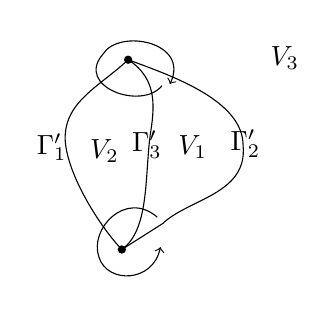
\begin{tikzpicture}[x=1cm,y=1cm]
\draw (1.08,2.56) .. controls (0.72,2.22) and (0.27,2.03) .. (0.28,1.55)
 .. controls (0.30,1.10) and (0.73,0.43) .. (1.00,0.15);
\draw (1.08,2.56) .. controls (1.47,2.31) and (1.41,1.93) .. (1.36,1.60)
 .. controls (1.29,1.07) and (1.35,0.40) .. (1.00,0.15);
\draw (1.08,2.56) .. controls (1.65,2.35) and (2.54,2.04) .. (2.54,1.47)
 .. controls (2.60,0.85) and (1.84,0.79) .. (1.52,0.48) -- (1.00,0.15);
\draw[->] (1.51,2.23) .. controls (1.25,1.91) and (0.40,2.22) .. (0.76,2.63)
 .. controls (0.96,2.96) and (1.87,2.79) .. (1.61,2.25);
\draw[->] (1.45,0.56) .. controls (1.05,0.91) and (0.58,0.41) .. (0.71,0.05)
 .. controls (0.82,-0.29) and (1.40,-0.27) .. (1.49,0.18);
\fill (1.08,2.56) circle (1.5pt); \fill (1.00,0.15) circle (1.5pt);
\node at (0.11,1.45) {$\Gamma'_1$}; \node at (0.78,1.40) {$V_2$};
\node at (1.32,1.48) {$\Gamma'_3$}; \node at (1.90,1.45) {$V_1$};
\node at (2.57,1.49) {$\Gamma'_2$}; \node at (3.07,2.58) {$V_3$};
\end{tikzpicture}}

$\Gamma'_i\qquad \alpha\in I$ ens \unsure{à|:} trois él.
chemin simple joignant les deux point de $\delta=\{x,y\}$

$\Gamma_i=\displaystyle\bigcup_{\underline{j}\in A-\{i\}}\Gamma'_j$
détermine un ens $B_i$ de card. 2 (\unsure{l'une|l'un} des 2 régions du \deleted{\unsure{pl.}}\inserted{$X$})

\[
 B=\coprod_{i\in I} B_i\qquad
 \text{\deleted{\unsure{:|.} \unsure{quotient|points|graphe} de 3 côtés}}
\]

Si $i\in I$ est donné, on lui associe $U_i$ la région de $\Gamma_i$ qui contient $\Gamma'_i-\delta$ \inserted{$=\Gamma_i^{\prime\circ}$}, d'où section de la \unsure{sur. quelle|surj. quelle|sur quelle}
\[
 B\simeq I\times\{0,1\},\qquad V_i
\]

\[
\begin{aligned}
 U_i&=\overset{\circ}{\Gamma}'_i\cup\bigcup_{j\in I\setminus\{i\}}U_j\\
 V_i&=\bigcap_{j\in I\setminus\{\unsure{i|1}\}}V_j
\end{aligned}
\qquad\Bigg/\qquad
\left\{\begin{gathered}
 V_1,V_2,V_3\\ \Gamma_1^\circ,\Gamma_2^\circ,\Gamma_3^\circ\\ \delta
\end{gathered}\right.
\quad
\left\{\begin{aligned}
 U_1&=V_2\cup V_3\cup\Gamma_1^\circ\\
 U_2&=V_3\cup V_1\cup\Gamma_2^\circ\\
 U_3&=V_1\cup V_2\cup\Gamma_3^\circ
\end{aligned}\right.
\]
\[
 U_i,U_j,\ U_k\qquad\Bigg/\qquad
\begin{aligned}
 V_3&=U_1\cap U_2\\
 V_2&=U_3\cap U_1\\
 V_1&=U_1\cap U_2
\end{aligned}
\quad
\left\{\begin{aligned}
 \Gamma_1&=\Gamma_2^\circ\cup\Gamma_3^\circ\cup\delta\\
 \Gamma_2&=\Gamma_3^\circ\cup\Gamma_{\unsure{1|2}}^\circ\cup\delta\\
 \Gamma_3&=\Gamma_1^\circ\cup\Gamma_2^\circ\cup\delta
\end{aligned}\right.
\]

$C$ courbe simple fermée dans surface connexe \deleted{$X$}$E$. Conditions équ.

a) card $\pi_0(\deleted{X}E-C)=2$ \quad (\uline{NB} on a tjrs card $\pi_{\unsure{0|{}}}(E-C)\le 2$)

b) $\exists$ ouvert $U\subset C$ tel que $\dot U(\overset{\text{dfn}}{=}\overline U-U)=C$ et que \deleted{\unsure{vide|de}}
$\overline U\ne E$ i.e. $V=\overline U-U\ne\emptyset$ i.e. $U\ne E\setminus C$.
% slanted
\margin{($U$ est alors une comp. connexe de $X-C$)}

c) (étant donné un disque $D_x$ assez petit \unsure{centré|\deleted{centré}} en $x\in C$\}, et un point $x'$ et un point $x''$ $\in D_x-D_x\cap C$ de part et d'autre de $D_x\cap C$ ....)
$x$ et $y$ n'appart\unsure{iennent|\deleted{iennent|ent}} \unsure{pas|ps.} à la $=$ composante connexe de $X-C$, i.e. $\nexists$ arc \unsure{dans|ds} $X-C$ joignant $x$ : $y$.
(Car $\{x,y\}\longrightarrow\pi_0(X-C)$ est surjectif ...)
